%%%%%%%%%%%%%%%%%%%%%%%%%%%%%%%%%%

\documentclass[a4paper,11pt]{article}
%\pdfoutput=1

%%%%%%%%%%%%%%%% Comment %%%%%%%%%%%%%%%%%%
%%% To add a comment, just add \YOURINITIALS{your comment}
\newcommand{\DA}[1]{\textbf{\textcolor{orange}{[DA: #1]}}}
\newcommand{\LG}[1]{\textbf{\textcolor{blue}{[LG: #1]}}}
\newcommand{\DR}[1]{\textcolor{red}{[DR: #1]}}
\newcommand{\MT}[1]{\textcolor{purple}{MT: #1]}}

%%%%%%%%%%%%%%%% Daniele %%%%%%%%%%%%%%%%%%

\usepackage[T1]{fontenc}
\usepackage[utf8]{inputenc}
\usepackage[english]{babel}
\usepackage{amsmath}
\usepackage{auxi/jheppub}

\usepackage{lmodern}
\usepackage{microtype}
\usepackage{amsfonts}
\usepackage{amssymb}
\usepackage{amsthm}
\usepackage{auxi/mhsetup}
\usepackage{auxi/mathtools}
\usepackage{graphicx}
\usepackage{pdfpages}
\usepackage{subfig}
\usepackage{multicol}
\usepackage{pdfpages}
\usepackage{float}
\usepackage{tikz-feynman}
\usepackage{lscape}
\usepackage{bm}
\usepackage{bbm}
\newtheorem{theorem}{Theorem}
\usepackage{aligned-overset}
%%%%%%%%%%%%%%%%%%%%%%%%%%%%%%%%%%%%%%%%%%%%%%%%%%%%%%%%%%
%%% To add a comment, just add \YOURINITIALS{your comment}
\newcommand{\EP}[1]{\textcolor{red}{[EP: #1]}}
\newcommand{\JB}[1]{\textcolor{purple}{[JB: #1]}}
\newcommand{\EM}[1]{\textcolor{cyan}{[EM: #1]}}
\newcommand{\BF}[1]{\textcolor{orange}{[BF: #1]}}
\newcommand{\AM}[1]{\textcolor{blue}{[AM: #1]}}
%%%%%%%%%%%%%%%%%%%%%%%%%%%%%%%%%%%%%%%%%%%%%%%%%%%%%%%%%%

%COLORS
\pgfdeclareverticalshading{rainbow}{100bp}
{color(0bp)=(red); color(25bp)=(red); color(35bp)=(yellow);
color(45bp)=(green); color(55bp)=(cyan); color(65bp)=(blue);
color(75bp)=(violet); color(100bp)=(violet)}
%Dark blue grey
\definecolor{DarkBlueGrey}{RGB}{76,94,107}
%Medium blue grey
\definecolor{MediumBlueGrey}{RGB}{110,135,153}
%Light blue grey
\definecolor{LightBlueGrey}{RGB}{134,163,184}
%Weak coupling orange
\definecolor{BalancedOrange}{RGB}{242,146,29}
%Strong coupling red
\definecolor{DarkRed}{RGB}{179,48,48}
%gluon line
\definecolor{SalmonPink}{RGB}{255,172,172}
%self-energy
\definecolor{SEColor}{RGB}{134,163,184}

%Circled numbers
\newcommand*\circled[1]{\tikz[baseline=(char.base)]{
            \node[shape=circle,draw,inner sep=2pt] (char) {#1};}}

%% DEFINE MATH COMMANDS
\newcommand{\op}[1]{\boldsymbol{#1}}
\newcommand{\de}{\mathrm d}
\newcommand{\sumint}{\ \mathclap{\displaystyle\int}\mathclap{\textstyle\sum}\ \ }
\newcommand{\Tr}{\operatorname{Tr}}
%Partial derivative
\newcommand{\pd}{\partial}
\newcommand{\spd}{\slashed{\partial}}
\newcommand{\sx}{\slashed{x}}
%Sign function
\DeclareMathOperator{\sgn}{sgn}
\DeclareMathOperator{\Disc}{Disc}
\DeclareMathOperator{\dDisc}{dDisc}
\DeclareMathOperator{\Res}{Res}
%Pfaffian
\newcommand{\Pf}{\text{Pf}\ }
%Super-Pfaffian
\newcommand{\SPf}{\text{SPf}\ }
%Dilogarithm
\newcommand{\Li}{{\normalfont\text{Li}}}
%Vev
\newcommand{\vvev}[1]{\langle\!\langle\, #1 \, \rangle\!\rangle}
\newcommand{\vev}[1]{\langle\, #1 \, \rangle}
%VarEpsilon
\def\veps{\varepsilon}

%%OTHER
\def\Op{{\mathcal{O}}}
\def\Oh{{\widehat{\mathcal{O}}}}
\newcommand{\Db}{\bar{\Delta}}
\newcommand{\Dh}{{\widehat{\Delta}}}
\newcommand{\zb}{{\bar{z}}}
\newcommand{\tlambda}{\tilde{\lambda}}
\newcommand{\tg}{\tilde{g}}
\newcommand{\vh}{\widehat{v}}
\newcommand\Fb{{\bar{F}}}
\newcommand{\nh}{\widehat{n}}
\newcommand{\AdSfive}{AdS$_5 \times S^5$}
\newcommand{\bh}{\widehat{b}}
\newcommand{\kh}{\widehat{k}}
\newcommand{\ch}{\widehat{c}}
\newcommand{\bt}{\tilde{b}}
\newcommand{\phat}{\widehat{p}}
\newcommand{\Qb}{\bar{Q}}
\newcommand{\Sb}{\bar{S}}
\newcommand{\sigmab}{\bar{\sigma}}
\newcommand{\Wt}{\tilde{W}}
\newcommand{\Zb}{\bar{Z}}
\newcommand{\alphah}{\hat{\alpha}}
\newcommand{\alphad}{\dot{\alpha}}
\newcommand{\betad}{\dot{\beta}}
\newcommand{\idh}{\hat{\mathds{1}}}
\newcommand{\id}{\mathds{1}}
\newcommand{\lambdah}{\hat{\lambda}}
\newcommand{\hh}{\hat{h}}
\newcommand{\fh}{\hat{f}}
\newcommand{\gammah}{\hat{\gamma}}
\newcommand{\Fh}{\hat{F}}
\newcommand{\ellb}{\bar{\ell}}
\newcommand{\Do}{{\Delta_{\Op}}}

\newcommand{\Ah}{\hat{\mathcal{A}}}
\newcommand{\Bh}{\hat{\mathcal{B}}}
\newcommand{\Ch}{\hat{\mathcal{C}}}
%\newcommand{\Dh}{\hat{\mathcal{D}}}
\newcommand{\Eh}{\hat{\mathcal{E}}}
%\newcommand{\Fh}{\hat{\mathcal{F}}}
\newcommand{\Gh}{\hat{\mathcal{G}}}
\newcommand{\Hh}{\hat{\mathcal{H}}}
\newcommand{\Ih}{\hat{\mathcal{I}}}
\newcommand{\Jh}{\hat{\mathcal{J}}}
\newcommand{\Kh}{\hat{\mathcal{K}}}
\newcommand{\Lh}{\hat{\mathcal{L}}}
\newcommand{\Mh}{\hat{\mathcal{M}}}
\newcommand{\Nh}{\hat{\mathcal{N}}}
%\newcommand{\Oh}{\hat{\mathcal{O}}}
\newcommand{\Ph}{\hat{\mathcal{P}}}
\newcommand{\Qh}{\hat{\mathcal{Q}}}
\newcommand{\Rh}{\hat{\mathcal{R}}}
\newcommand{\Sh}{\hat{\mathcal{S}}}
\newcommand{\Th}{\hat{\mathcal{T}}}
\newcommand{\Uh}{\hat{\mathcal{U}}}
\newcommand{\Vh}{\hat{\mathcal{V}}}
\newcommand{\Wh}{\hat{\mathcal{W}}}
\newcommand{\Xh}{\hat{\mathcal{X}}}
\newcommand{\Yh}{\hat{\mathcal{Y}}}
\newcommand{\Zh}{\hat{\mathcal{Z}}}

\newcommand{\OR}{\sigma}
% \newcommand{\OR}{\Omega_\text{R}}

\def\Am{{\mathcal{A}}}
\def\Bm{{\mathcal{B}}}
\def\Cm{{\mathcal{C}}}
\def\Dm{{\mathcal{D}}}
\def\Em{{\mathcal{E}}}
\def\Fm{{\mathcal{F}}}
\def\Gm{{\mathcal{G}}}
\def\Hm{{\mathcal{H}}}
\def\Im{{\mathcal{I}}}
\def\Jm{{\mathcal{J}}}
\def\Km{{\mathcal{K}}}
\def\Lm{{\mathcal{L}}}
\def\Mm{{\mathcal{M}}}
\def\Nm{{\mathcal{N}}}
\def\Om{{\mathcal{O}}}
\def\Pm{{\mathcal{P}}}
\def\Qm{{\mathcal{Q}}}
\def\Rm{{\mathcal{R}}}
\def\Sm{{\mathcal{S}}}
\def\Tm{{\mathcal{T}}}
\def\Um{{\mathcal{U}}}
\def\Vm{{\mathcal{V}}}
\def\Wm{{\mathcal{W}}}
\def\Xm{{\mathcal{X}}}
\def\Ym{{\mathcal{Y}}}
\def\Zm{{\mathcal{Z}}}

\def\Ads{{\mathds{A}}}
\def\Bds{{\mathds{B}}}
\def\Cds{{\mathds{C}}}
\def\Dds{{\mathds{D}}}
\def\Eds{{\mathds{E}}}
\def\Fds{{\mathds{F}}}
\def\Gds{{\mathds{G}}}
\def\Hds{{\mathds{H}}}
\def\Ids{{\mathds{I}}}
\def\Jds{{\mathds{J}}}
\def\Kds{{\mathds{K}}}
\def\Lds{{\mathds{L}}}
\def\Mds{{\mathds{M}}}
\def\Nds{{\mathds{N}}}
\def\Ods{{\mathds{O}}}
\def\Pds{{\mathds{P}}}
\def\Qds{{\mathds{Q}}}
\def\Rds{{\mathbb{R}}}
\def\Sds{{\mathds{S}}}
\def\Tds{{\mathds{T}}}
\def\Uds{{\mathds{U}}}
\def\Vds{{\mathds{V}}}
\def\Wds{{\mathds{W}}}
\def\Xds{{\mathds{X}}}
\def\Yds{{\mathds{Y}}}
\def\Zds{{\mathds{Z}}}

%% HELP FUNCTION FOR DIAGRAMS: gluon lines are symmetric
\newif\ifstartcompletesineup
\newif\ifendcompletesineup
\pgfkeys{
    /pgf/decoration/.cd,
    start up/.is if=startcompletesineup,
    start up=true,
    start up/.default=true,
    start down/.style={/pgf/decoration/start up=false},
    end up/.is if=endcompletesineup,
    end up=true,
    end up/.default=true,
    end down/.style={/pgf/decoration/end up=false}
}
\pgfdeclaredecoration{complete sines}{initial}
{
    \state{initial}[
        width=+0pt,
        next state=upsine,
        persistent precomputation={
            \ifstartcompletesineup
                \pgfkeys{/pgf/decoration automaton/next state=upsine}
                \ifendcompletesineup
                    \pgfmathsetmacro\matchinglength{
                        0.5*\pgfdecoratedinputsegmentlength / (ceil(0.5* \pgfdecoratedinputsegmentlength / \pgfdecorationsegmentlength) )
                    }
                \else
                    \pgfmathsetmacro\matchinglength{
                        0.5 * \pgfdecoratedinputsegmentlength / (ceil(0.5 * \pgfdecoratedinputsegmentlength / \pgfdecorationsegmentlength ) - 0.499)
                    }
                \fi
            \else
                \pgfkeys{/pgf/decoration automaton/next state=downsine}
                \ifendcompletesineup
                    \pgfmathsetmacro\matchinglength{
                        0.5* \pgfdecoratedinputsegmentlength / (ceil(0.5 * \pgfdecoratedinputsegmentlength / \pgfdecorationsegmentlength ) - 0.4999)
                    }
                \else
                    \pgfmathsetmacro\matchinglength{
                        0.5 * \pgfdecoratedinputsegmentlength / (ceil(0.5 * \pgfdecoratedinputsegmentlength / \pgfdecorationsegmentlength ) )
                    }
                \fi
            \fi
            \setlength{\pgfdecorationsegmentlength}{\matchinglength pt}
        }] {}
    \state{downsine}[width=\pgfdecorationsegmentlength,next state=upsine]{
        \pgfpathsine{\pgfpoint{0.5\pgfdecorationsegmentlength}{0.5\pgfdecorationsegmentamplitude}}
        \pgfpathcosine{\pgfpoint{0.5\pgfdecorationsegmentlength}{-0.5\pgfdecorationsegmentamplitude}}
    }
    \state{upsine}[width=\pgfdecorationsegmentlength,next state=downsine]{
        \pgfpathsine{\pgfpoint{0.5\pgfdecorationsegmentlength}{-0.5\pgfdecorationsegmentamplitude}}
        \pgfpathcosine{\pgfpoint{0.5\pgfdecorationsegmentlength}{0.5\pgfdecorationsegmentamplitude}}
}
    \state{final}{}
}

\newcommand{\dx}{\text{d}x}
\newcommand{\red}[1]{\textcolor{red}{#1}}
\newcommand{\green}[1]{\textcolor{green}{#1}}
\newcommand{\warning}[1]{{\red{ {#1}}}}
\newcommand{\reminder}[1]{({\green{ {#1}}})}
\newcommand{\blue}[1]{\textcolor{blue}{#1}}
\newcommand{\sourav}[1]{{\blue{ {#1}}}}
\def\bra#1{%
  \left\langle\smash{#1}{\vphantom1}\right|}
\def\ket#1{%
  \left|\smash{#1}{\vphantom1}\right\rangle}
%\def\eq#1{Eq.~(\ref{#1})}
\newcommand{\secn}[1]{Section~\ref{#1}}
\newcommand{\be}{\begin{equation}}
\newcommand{\ee}{\end{equation}}
\newcommand{\beq}{\begin{eqnarray}}
\newcommand{\eeq}{\end{eqnarray}}
\newcommand{\bea}{\begin{eqnarray}}
\newcommand{\eea}{\end{eqnarray}}
\newcommand{\nn}{\nonumber}
\newcommand{\e}{\epsilon}
\newcommand{\ord}{{\cal O}}
\newcommand{\as}{\alpha_s}
\newcommand{\daniele}[1]{\textbf{\textcolor{orange}{[DA: #1]}}}

%%%%%%%%%%%%%%%% Adam %%%%%%%%%%%%%%%%%%

\usepackage[T1]{fontenc} % if needed
\newcommand{\oD}{\bar{D}}
\newcommand{\oE}{\bar{E}}
\newcommand{\oR}{\bar{R}}
\newcommand{\oW}{\bar{W}}
\newcommand{\oG}{\bar{\Gamma}}
\newcommand{\oK}{\mathring{K}}
\newcommand{\II}{\mathrm{I\hspace{-0.02cm} I}}
\newcommand{\oII}{\mathring{\II}}
\newcommand{\CA}{\mathcal{A}}
\newcommand{\CB}{\mathcal{B}}
\newcommand{\CC}{\mathcal{C}}
\newcommand{\CD}{\mathcal{D}}
\newcommand{\CE}{\mathcal{E}}
\newcommand{\CF}{\mathcal{F}}
\newcommand{\CH}{\mathcal{H}}
\newcommand{\CI}{\mathcal{I}}
\newcommand{\CJ}{\mathcal{J}}
\newcommand{\CK}{\mathcal{K}}
\newcommand{\CL}{\mathcal{L}}
\newcommand{\CM}{\mathcal{M}}
\newcommand{\CN}{\mathcal{N}}
\newcommand{\CO}{\mathcal{O}}
\newcommand{\CP}{\mathcal{P}}
\newcommand{\CQ}{\mathcal{Q}}
\newcommand{\CT}{\mathcal{T}}
\newcommand{\CW}{\mathcal{W}}
\newcommand{\CX}{\mathcal{X}}
\newcommand{\CZ}{\mathcal{Z}}
\newcommand{\Ff}{\mathfrak{f}^{\text{\tiny bdy}}}
\newcommand{\Ffbulk}{\mathfrak{f}^{\text{\tiny blk}}}
\newcommand{\FF}{\mathfrak{F}^{\text{\tiny bdy}}}
\newcommand{\CPS}{\CP_\Sigma}
\newcommand{\CPM}{\CP_\CM}
\newcommand{\tCB}{\tilde{\CB}}
\newcommand{\g}{\gamma}
\newcommand{\s}{\sigma}
\DeclareMathOperator{\sech}{sech}
\DeclareMathOperator{\csch}{csch}

\newcommand{\w}{\omega}
\renewcommand{\de}{\delta}
\newcommand{\dw}{\delta\omega_1}
\newcommand{\dww}{\delta\omega_2}
\newcommand{\oB}{\mathring{\Box}}
\newcommand\eq[1]{eq.~(\ref{eq:#1})}
\newcommand{\ul}{\underline}
\newcommand{\G}{\Gamma}
\newcommand{\iu}{\text{i}}
\newcommand{\gYM}{g_{\text{\tiny YM}}}
\newcommand{\discmo}{\underset{\xi<-1}{\text{disc}}}
\newcommand{\discmoz}{\underset{-1<\xi<0}{\text{disc}}}
\newcommand{\Ffbdy}{\mathfrak{f}^{\text{\tiny bdy}}}

\newcommand{\bD}{\bar{D}}
\newcommand{\Fcl}{F^\mathrm{cl}}
\newcommand{\Acl}{A^\mathrm{cl}}
\newcommand{\pcl}{\varphi^\mathrm{cl}}
\newcommand{\nabladef}{\nabla_\mathrm{3d}}
\newcommand{\p}{\partial}
\newcommand{\vp}{\varphi}
\newcommand{\bP}{\bar{\Phi}}
\newcommand{\bPs}{\bar{\Psi}}
\newcommand{\Pcl}{\Phi^\mathrm{cl}}
\newcommand{\bPcl}{\bar{\Phi}^\mathrm{cl}}
\newcommand{\bAp}{\bar{A}_\perp}
\newcommand{\Ap}{A_\perp}
\newcommand{\bap}{\bar{a}_\perp}
\newcommand{\ap}{a_\perp}
\newcommand{\Fdef}{\mathfrak{f}^\mathrm{def}}
\newcommand{\Fbdy}{\mathfrak{f}^\mathrm{bdy}}

\DeclareMathOperator{\uu}{\mathfrak{u}}
\DeclareMathOperator{\su}{\mathfrak{su}}
\DeclareMathOperator{\psu}{\mathfrak{psu}}
\DeclareMathOperator{\so}{\mathfrak{so}}
\DeclareMathOperator{\iso}{\mathfrak{iso}}
\DeclareMathOperator{\osp}{\mathfrak{osp}}
\DeclareMathOperator{\MPS}{\text{MPS}}

\renewcommand{\d}{\text{d}}


%%%%%%%%%%%%%%%%%%%%%%%%%%%%%%%%%%

% --------------------------------------------------
% Title and Author Info
% --------------------------------------------------

\title{Free Water Access Under Urban Heat Stress: Mapping Drinking Fountain Accessibility and Climate Vulnerability in Italian Cities}

%%% Authors

\author[a]{Daniele Artico,}
\author{Ludovica Gatti,}
\author{Davide Ravaglia,}
\author{Matilde Torrassa}

%%% Affiliation

\affiliation[a]{Dipartimento SMFI, Universit\`a di Parma, Viale G.P. Usberti 7/A, 43100, Parma, Italy and INFN
Gruppo Collegato di Parma}

%%% E-mail addresses

\emailAdd{daniele.artico@unipr.it}

\abstract{This project evaluates whether Italian cities’ free public drinking-water infrastructure is spatially aligned with present and future heat-health risk. Combining mapped fountains, walking-distance accessibility, heatwave indicators, urban heat exposure, demographic vulnerability, and available health-burden data, the project identifies neighborhoods where climate adaptation through free water access is insufficient.}

\begin{document}
\maketitle
\noindent
\section{Project pitch}

%General background: what we know
Heatwaves are increasingly becoming a major urban public-health risk: the years 2015–2025 constitute the eleven warmest consecutive years since global temperature records began. 
Thousands of additional deaths are being recorded every year in Europe due to events of extreme heat, and climate change is expected to make heatwaves more frequent and more intense.
However, urban heat risk is not only meteorological. 
Several factors contribute to making heatwaves more survivable or, in the worst case, less managable from a public healt point of view.
These factors include, and are not limited to: exposure, age, health, income, mobility, housing, shade, and access to cooling resources.
The European Union Climate Adaptation Strategy has already established that providing free access to water for both drinking and cooling purposes is fundamental to address extreme heat in cities, especially during heatwaves.
Drinking fountains can reduce heat-stress risk and support hydration in public space; and existing studies already mention heat-stroke reduction as one core benefit.
Moreover, fountains can also have positive social effects: they can be used as meeting places fostering community ownership of a public space. Heat-adaptation infrastructure is often studied through cooling centers, green space, shade, and shelters.
On the other hand, research on public drinking fountains in the scientific literature is fairly limited, and we did not identify any sistematic study involving Italy.\\
 
%Specific background: what is missing?
The existing literature has mostly focused on single cities, with the declared intent of mapping sites for priority improvement and demographic characteristics of communities near the water fountains.
A public health approach has been applied to cooling-center accessibility, which has been studied for heat-vulnerable populations, including the variables of walking-distance and transport access. Heat vulnerability stands at the core of the analysis performed for the city on Vancouver, with the purpose of creating an equitable drinking fountain placement framework. 
What is missing for Italy is a national (or multi-city) analysis connecting public drinking fountains to population-weighted accessibility, with a particular focus on present heatwave exposure and future heat projections.\\

%The gap we want to fill
This research gap undermines our understanding of the degree of adaptation of free public drinking-water infrastructure to current and future climate needs. 
In other words, we do not know whether areas most exposed to heatwaves are also areas with poor public water access. 
Additionally, we do not know whether elderly or vulnerable populations are systematically better or worse served than the general population. T
he project fills this gap by treating public drinking-water fountains as measurable climate-adaptation infrastructure and testing whether their accessibility is spatially aligned with heatwave vulnerability.\\
%
\begin{figure}
\centering
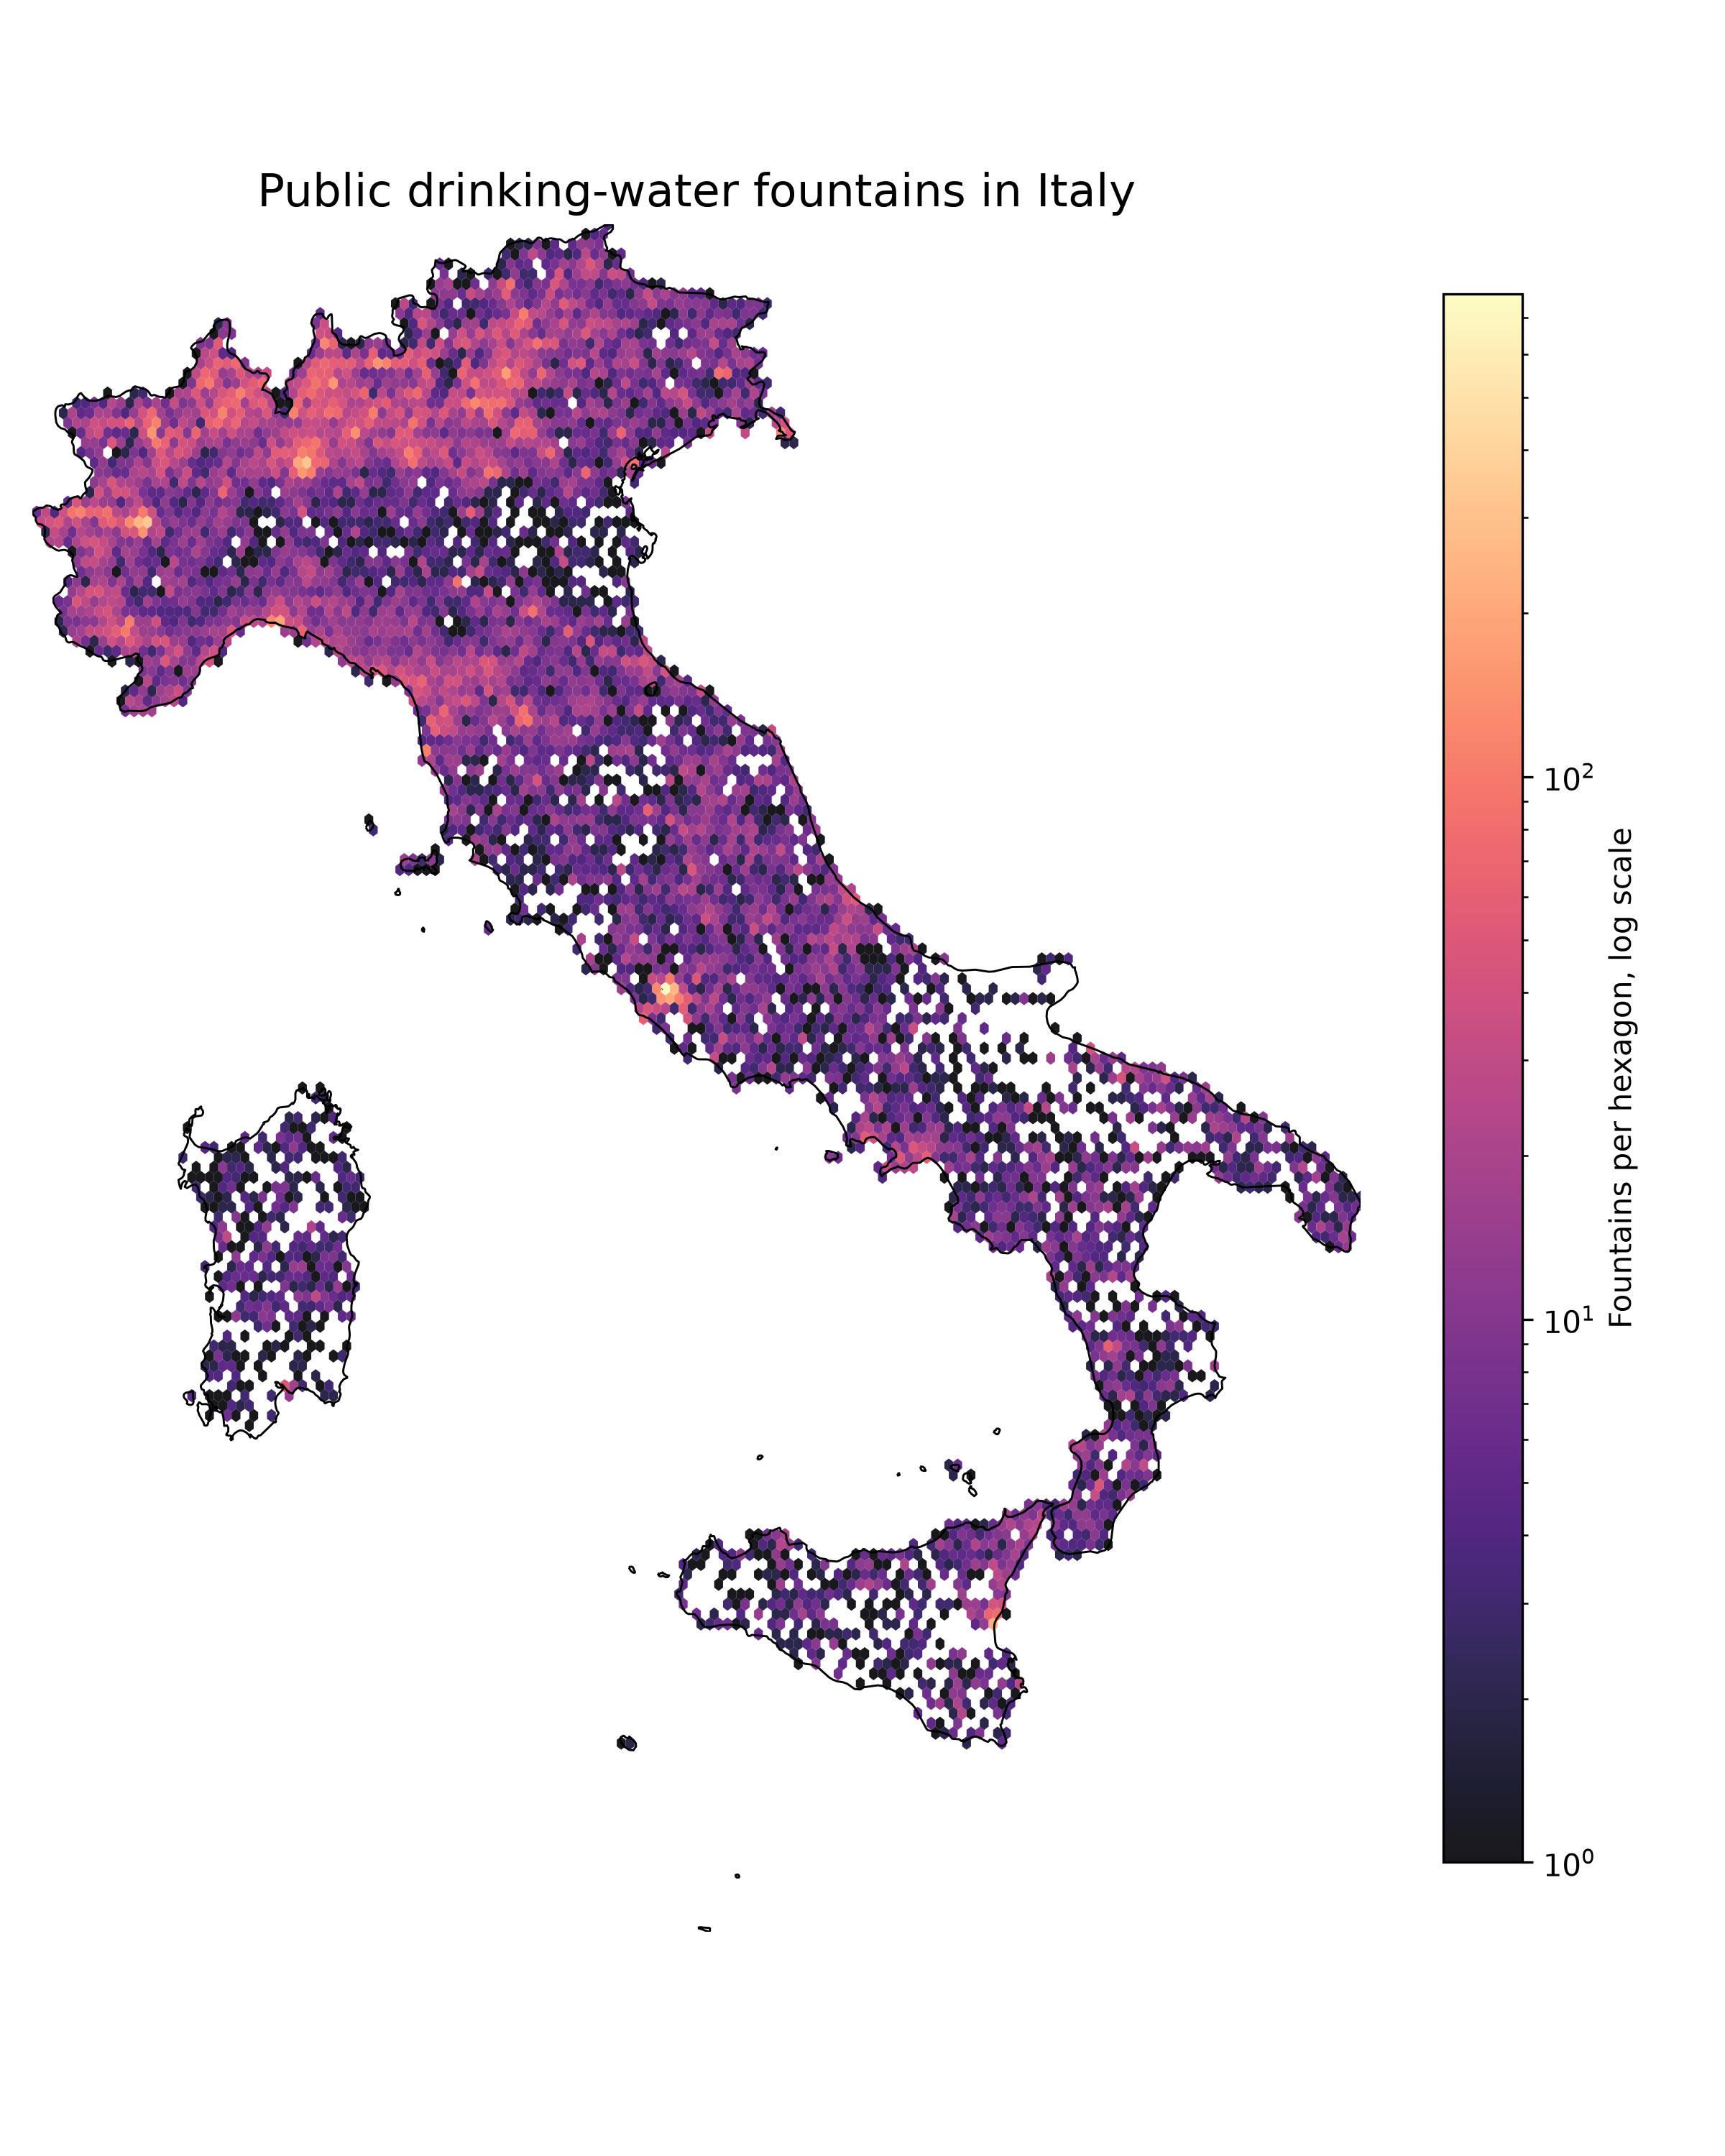
\includegraphics[scale=0.4]{../code_folder/fountain_density_italy_pitch.png}
\caption{Map of fountain distribution in Italy. Data were collected from the project \href{https://github.com/matitalatina/fontanelle}{Fontanelle in Italia}.}
\label{fig:fount_dens}
\end{figure}
%

%Preliminary work: part of the answer
%You have already collected geolocated fountain data for Italy.
Foundational to this work is the availability of data on public fountains distribution in Italy. 
Our project relies on Open Street Map data, collected through the project \href{https://github.com/matitalatina/fontanelle}{Fontanelle in Italia} available on GitHub. 
A preliminary analisys produced a national fountain-density map shown in Fig~\ref{fig:fount_dens}. 
A second key dataset is the population distribution in Italy, which we obtained from the WorldPop gridded population data. 
Combined, these two datasets give access to a first accessibility metric: population within 250 m of a drinking-water fountain, presented in Fig.~\ref{fig:250m_avail}. 
This preliminary pattern clearly shows spatially uneven accessibility with visible underserved areas, which strenghtens the motivation for this research.\\

%
\begin{figure}
\centering
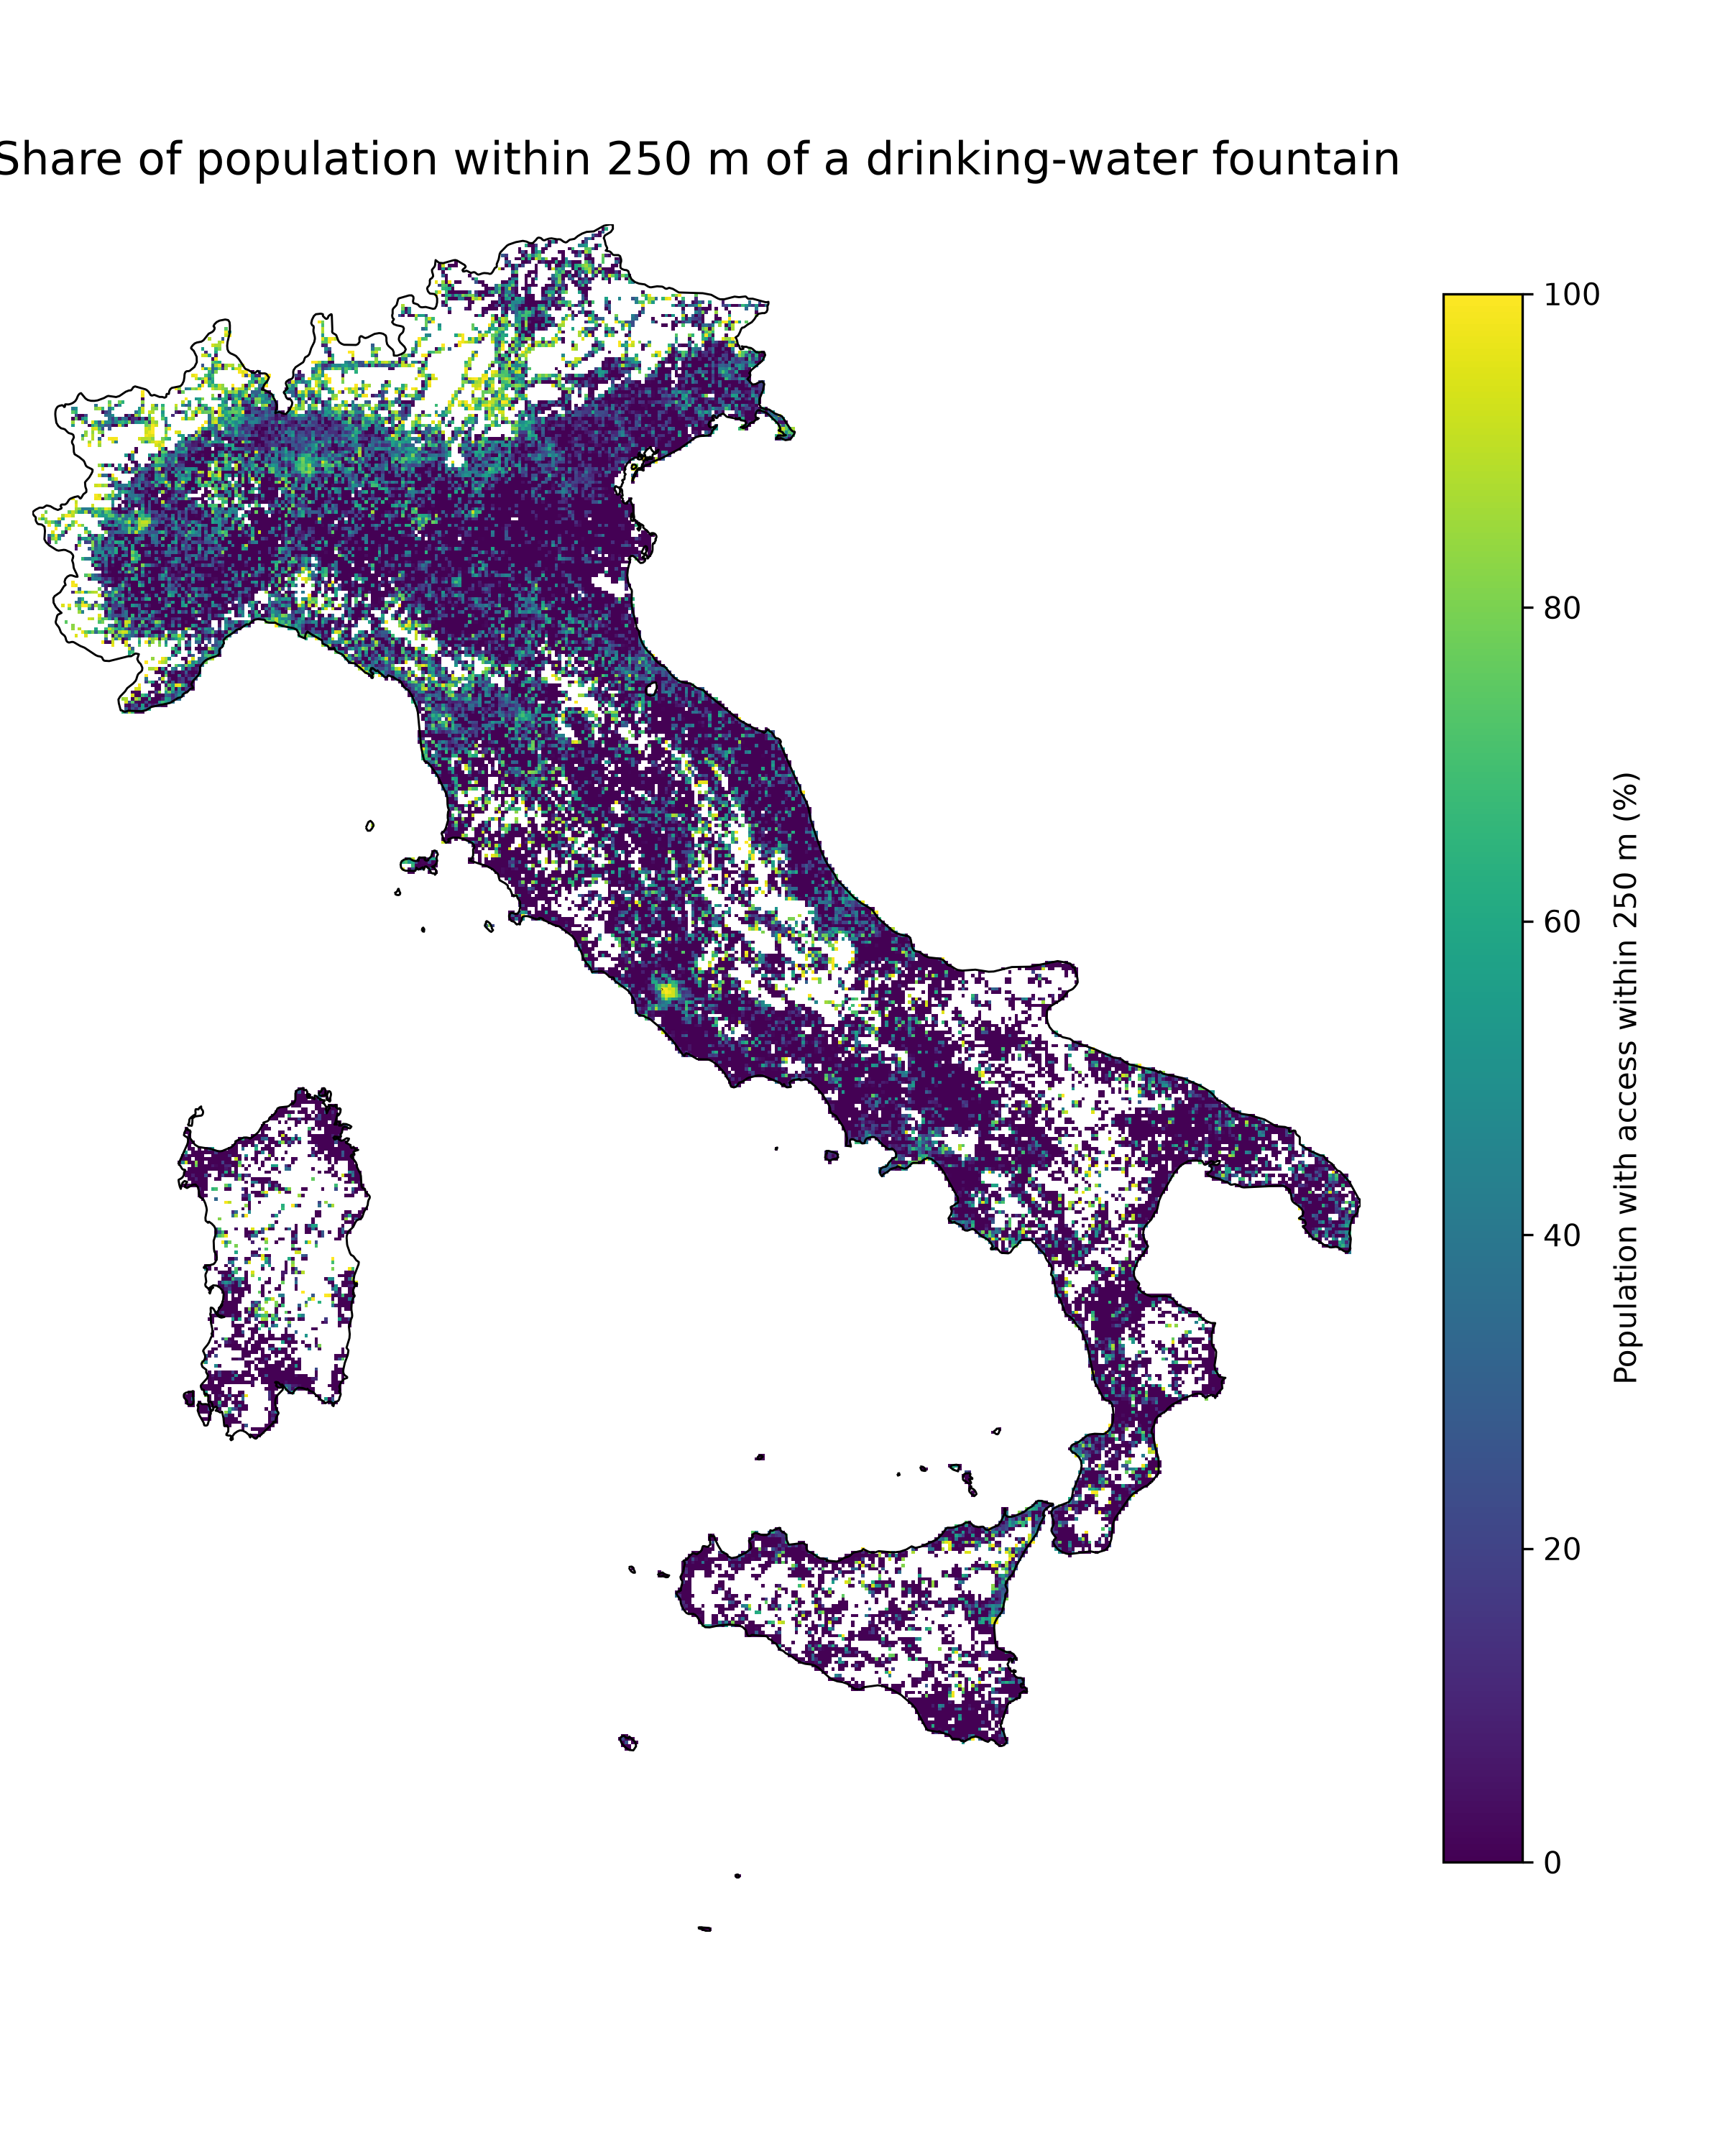
\includegraphics[scale=0.4]{../code_folder/share_population_within_250m_of_fountain.png}
\caption{Map of fountain availability within 250m in Italy.}
\label{fig:250m_avail}
\end{figure}
%

% Central hypothesis and testing
Our core hypothesis is that public drinking-water fountains are an under-recognized form of urban heat-adaptation infrastructure, and in Italy their spatial distribution is not aligned with present and future heat vulnerability. 
We plan to test our hypothesis across three layers, focused on accessibility, heat exposure and vulnerability. 
A final stage will evaluate the spatial mismatch to identify priority areas for public drinking-water adaptation.
The first layer will expand on the preliminary analysis by repeating the analysis for residents within 500m from a fountain and the median distance to nearest fountain for each cell. 
The share of people within a certan distance may serve as measurement to test against regression model prediction based on the heat sensitivity built in the second layer.  
The heat exposure layer is built from CERRA data and consists in establishing the current heatwave frequency, intensity, and the frequency of tropical nights. Future exposure will be established using data from CMIP6 Climate Projections for the 1985–2100 Period, using statistical downscaling over Italy using EQM.
The third layer of the analysis will deal with vulnerability metrics, including share of elderly population, socioeconomic conditions, outdoor worker presence and health indicators, if accessible.\\

%If the hypothesis is right, what do we learn?
If the analysis supports our hypothesis, we confirm that Italy has spatial inequalities in free public water access exposing some populations to enhanced heatwave sentitivity.
The project would introduce a reproducible indicator of hydration accessibility that municipalities can use to identify priority locations for new fountains, framed as low-cost, actionable climate-adaptation infrastructure.
%If the hypothesis is wrong, what do we learn?
The project remains interesting even in the case that data do not support our hypothesis: some cities may offer examples of good adaptation practice, and the developed method can identify which municipalities are already successful.
The project would shift from adaptation gap to best-practice mapping, quantifying an adaptation asset that is usually invisible.\\

In both cases, the project would have several beneficial impact on the scientific and policy-maker communities, by connecting climate risk to everyday urban infrastructure.
It would provide a concrete, policy-relevant map of public water accessibility, while helping municipalities prioritize new fountain installation.
Local communities would receive data support for heatwave adaptation planning, reinforcing environmental-justice arguments; scientists and academics would benefit from the open code and reproducible spatial indicators.

\section{Introduction}

\section{Fountain accessibility}
Share of population within 250m or 500m walking distance of a fountain.
\begin{itemize}
\item	fountains per $km^2$
\item	fountains per 1000 residents
\item	fountains per 1000 elderly residents
\item	median walking distance to nearest fountain
\item	share of residents within 250 m or 500 m
\item	share of vulnerable residents within 250 m ot 500 m
\item	correlation with average income distribution
\end{itemize}

\section{Heat exposure and vulnerability}
For each city or neighborhood, compute:
\begin{itemize}
\item	historical heatwave days;
\item	tropical nights;
\item	annual maximum temperature;
\item	projected increase in maximum temperature;
\item	projected increase in heatwave days;
\item	elderly population share;
\item	socioeconomic deprivation;
\item	impervious surface;
\item	tree cover;
\item	urban heat island intensity.
\end{itemize}
\section{Data analysis}
Compute correlation matrices between variables in the previous sections. We expect there may be non-uniform mapping effects: we could repeat the analysis for urban areas such as
\subsection{Turin}
\subsection{Milan}
\subsection{Rome}
\subsection{Naples}
%\clearpage
%\section*{Bibliography}
%\addcontentsline{toc}{section}{Bibliography}
\appendix


\acknowledgements


\bibliography{auxi/refs.bib}
\bibliographystyle{auxi/JHEP}


\end{document}
